% Numbers come from artifacts/reported_results/2026-09-30-reward-service/ (see its README).
% Generated by artifacts/reported_results/2026-09-30-reward-service/generate.py; do not edit.
\newcommand{\RSLocalBackends}{19}
\newcommand{\RSServiceScorers}{13}
\newcommand{\RSSmallBase}{126.8}
\newcommand{\RSSmallSerial}{111.5}
\newcommand{\RSSmallOverlap}{106.9}
\newcommand{\RSSmallSerialSaving}{12.1\%}
\newcommand{\RSSmallOverlapSaving}{15.7\%}
\newcommand{\RSLargeBase}{179.7}
\newcommand{\RSLargeSerial}{145.0}
\newcommand{\RSLargeOverlap}{146.3}
\newcommand{\RSLargeSerialSaving}{19.3\%}
\newcommand{\RSLargeSerialMin}{144.4}
\newcommand{\RSLargeSerialMax}{146.0}
\newcommand{\RSLargeOverlapMin}{144.3}
\newcommand{\RSLargeOverlapMax}{149.1}
\newcommand{\RSSmallWholeService}{3.08}
\newcommand{\RSSmallMicroService}{1.20}
\newcommand{\RSSmallWholeWork}{24.6}
\newcommand{\RSSmallMicroWork}{38.5}
\newcommand{\RSSmallWholeWaitMax}{24.6}
\newcommand{\RSSmallSerialFirstWaitMax}{9.6}
\newcommand{\RSSmallSerialLaterWait}{1.3}
\newcommand{\RSSmallOverlapIdle}{44.3}
\newcommand{\RSLargeWholeService}{9.61}
\newcommand{\RSLargeWholeWork}{76.9}
\newcommand{\RSLargeFirstArrival}{24.3}
\newcommand{\RSLargeSerialService}{3.76}
\newcommand{\RSLargeSerialWork}{120.4}
\newcommand{\RSLargeSerialWorkMin}{119.7}
\newcommand{\RSLargeSerialWorkMax}{121.4}
\newcommand{\RSLargeOverlapWork}{121.8}
\newcommand{\RSLargeOverlapWorkMin}{119.5}
\newcommand{\RSLargeOverlapWorkMax}{124.5}
\newcommand{\RSLocalBase}{56.0}
\newcommand{\RSLocalSerial}{52.4}
\newcommand{\RSSmallShallowBase}{64.6}
\newcommand{\RSSmallShallowSerial}{59.6}
\newcommand{\RSSmallShallowSplit}{69.6}
\newcommand{\RSLargeShallowBase}{98.5}
\newcommand{\RSLargeShallowSerial}{86.9}
\newcommand{\RSLargeShallowSplit}{113.1}
\newcommand{\RSTrainRemoteNoCollect}{192.2}
\newcommand{\RSTrainRemoteCollect}{178.1}
\newcommand{\RSTrainLocalNoCollect}{58.0}
\newcommand{\RSTrainLocalCollect}{54.5}
\newcommand{\RSLargeWholePerPair}{0.30}
\newcommand{\RSLargeMicroPerPair}{0.47}
\newcommand{\RSSmallWholePerPair}{0.096}
\newcommand{\RSSmallMicroPerPair}{0.150}
\newcommand{\RSMpsThreeLight}{24.9\%}
\newcommand{\RSMpsTwoLight}{9.6\%}


\section{Reward Serving and Generation--Reward Overlap}
\label{sec:reward}

Reward is the one role of the feedback program whose cost the policy does not determine.
A contrastive preference model scores a batch in well under a second; a vision--language judge with tens of billions of parameters can take as long as the generation it evaluates, needs a different software stack from the trainer, and may not fit beside the policy on one accelerator.
\system therefore fixes what a reward \emph{is} at the trajectory boundary and leaves where it runs, in which environment, and when it is called relative to generation as separate execution choices.

\paragraph{Source scope.}
This section describes UniRL commit \texttt{651490e} (2026-09-30), which is later than the design-audit commit used elsewhere in the paper.
The shared-GPU mechanism of Section~\ref{sec:reward-mps} is an open pull request (\#492 at \texttt{8bb4119}) and is not part of that commit.
The measurements in Section~\ref{sec:reward-results} lie outside the E0--E6 programme; their per-rollout records and generator are under \codepath{artifacts/reported\_results/2026-09-30-reward-service/}.

\subsection{One scoring contract over many scorers}
\label{sec:reward-contract}

A trainer calls one method, \texttt{score\_and\_attach}, on the reward role.
The call is scattered over tree-complete shards like any other distributed method (Section~\ref{sec:execution}); on each shard it assembles a typed request from the trajectory, asks exactly one backend for scores, and returns a new trajectory whose frontier carries a scalar reward and named component rewards per row.
The request holds the frontier's decoded values, the non-text values of earlier turns as conditioning (for example the source image of an edit), the original and the generation prompt, and the sample and group identifiers.
A backend states which prompt it scores against; after a rewrite stage the two differ, and the choice decides whether the reward measures fidelity to the user's request or to the rewritten text.

The role refuses to be a silent source of bad credit.
It rejects a frontier that already carries rewards, raises when any row fails or returns a non-finite score instead of substituting zero, and sets the reward of a free-length autoregressive trace that ran into its token limit to zero, or applies a length penalty, as configured.
It also rejects a training reward that gives prompt-to-video alignment no weight, since an audio--video agreement score alone can be raised by collapsing both streams; such a score remains available for evaluation.
A group-normalized advantage spreads one corrupted reward over every sibling in its group, which is why these cases stop the step.

Table~\ref{tab:reward-scorers} lists what currently implements the contract: \RSLocalBackends{} in-process backends and \RSServiceScorers{} scorers registered in the standalone reward service.
They cover contrastive and preference models such as CLIP, PickScore, HPS and ImageReward~\citep{radford2021clip,kirstain2023pickapic,wu2023hpsv2,ma2025hpsv3,xu2023imagereward}, vision--language judges for composition, rendered text and instruction-guided editing~\citep{kamath2025geneval2,wu2025editreward,luo2025editscore}, video and audio--video alignment models, and text graders for reasoning workloads.
A remote backend can request a panel of scorers for each row and reduce it by a weighted sum, mean, minimum or maximum; the individual scores stay attached as components for logging.
Presence in the table means that the code path exists and is reachable from a recipe; it is not evidence that every scorer has been exercised in training.

\begin{table}[H]
\caption{Reward implementations at commit \texttt{651490e}, by the output they score. Names are registry keys. $^{\ast}$Registered but disabled in the example service configuration.}
\label{tab:reward-scorers}
\centering
\small
% Generated by artifacts/reported_results/2026-09-30-reward-service/generate.py; do not edit.
\begin{tabularx}{\textwidth}{@{}L{0.14\textwidth}YY@{}}
\toprule
Output scored & In-process backends & Reward-service scorers \\
\midrule
Image & \texttt{clip}, \texttt{pickscore}, \texttt{hpsv2}, \texttt{hpsv3}, \texttt{hpsv3pp}, \texttt{image\_reward}, \texttt{ocr}, \texttt{geneval2} & \texttt{clip}, \texttt{pickscore}, \texttt{imagereward}, \texttt{hpsv2}, \texttt{hpsv3}, \texttt{unified\_reward}, \texttt{geneval2}, \texttt{geneval}$^{\ast}$, \texttt{ocr}, \texttt{wise} \\
Image editing & -- & \texttt{editreward}, \texttt{editscore} \\
Video & \texttt{videopickscore}, \texttt{videoclipdelta}, \texttt{videoalign}, \texttt{video} & \texttt{videoalign}$^{\ast}$ \\
Audio & \texttt{clap} & -- \\
Audio--video & \texttt{imagebind}, \texttt{t2av\_composite} & -- \\
Text & \texttt{math\_verify}, \texttt{mc\_exact\_match}, \texttt{llm\_judge} & -- \\
Routing & \texttt{per\_domain} & -- \\
\bottomrule
\end{tabularx}

\end{table}

\subsection{Where a scorer runs}
\label{sec:reward-placement}

The same contract is served from four places, which differ in what they isolate.

\paragraph{In the policy's workers.}
An in-process backend loads the scorer in the worker that also hosts training and rollout roles.
Its memory is governed by the residency policy of Section~\ref{sec:lifecycle}: one choice per role states whether the trainer, the rollout engine and the reward keep their weights on the accelerator while idle, and a planner issues only the transitions that change that state.
A reward phase that follows generation therefore inherits an already parked trainer instead of moving it again.

\paragraph{On a reward slab.}
A placement fraction carves the tail of the device pool into a disjoint slab for the reward role.
Scoring is scattered over that slab's workers and the decoded values reach it as tensor references, so a heavier scorer stops competing with the policy for memory while the job remains one program.

\paragraph{In a managed child process.}
Scorers built on a serving engine or on pinned library versions often cannot be imported into the trainer's environment.
A managed backend starts one scorer process per reward worker with its own Python interpreter, hands it a listening loopback socket and that worker's single visible device, and speaks HTTP to it.
The protocol is deliberately strict.
Requests are sent in bounded chunks independent of the shard size.
Every item carries its sample, group, source rank, policy version and scorer version, and the child must echo them.
An idempotency key derived from those fields and a fingerprint of the payload lets a retried request return the cached result instead of scoring twice.
The child serializes scoring with its lifecycle operations and refuses non-finite outputs.
The parent can keep the scorer resident or bring it onto the device only for the duration of each call.
A child may host an entire vLLM engine~\citep{kwon2023vllm}: for the EditScore judge, the merged integration reports that parking takes 5.1\,s and leaves 1.0\,GB of 47\,GB on the device, that waking takes 0.3\,s, and that scores are bit-identical across the cycle.
Managed children currently accept image and image-editing requests only.

\paragraph{In a standalone service.}
A separate reward service places a gateway in front of Ray worker groups~\citep{moritz2018ray}.
Each configured reward is a group of replica actors that reserve their own devices and install their own package set on first start.
The gateway decodes a batch once, buckets its items by requested reward, issues one actor call per reward with round-robin replica choice, and awaits each reward under its own timeout.
A reward that fails is reported per item and per reward next to the scores that succeeded, so one scorer cannot turn a whole batch into an error; the client treats any missing score as a failure of that row.
The per-scorer environments of the gateway share the cluster's interpreter and PyTorch build, which is the limit that the managed child removes.
The single-scorer server used for managed children can also be started by hand on another node, which is how the judges of Section~\ref{sec:reward-results} were served.

\subsection{Overlapping reward with generation}
\label{sec:reward-overlap}

In the synchronous diffusion loop the driver first has every data-parallel rank generate its whole shard and only then dispatches scoring.
With a remote judge this wastes time twice: the training node idles while the judge works, and all ranks' requests reach the judge at the same instant and queue behind one another.

An optional worker-side role, \texttt{RewardStack}, changes the unit of work instead of the contract.
It is built on the same worker as the rollout engine and the reward role, slices the frontier of its shard into micro-batches of a configured number of rows, and for each micro-batch calls the engine and then the reward in process.
The scored parts are concatenated in the original row order, so group membership and credit assignment are unchanged, and the driver skips its own reward phase.
A micro-batch may be a single row; if the engine packs a whole sibling group into one request, the micro-batch is extended to the end of the group it would otherwise split. (Section~\ref{sec:fidelity-pack} removes that floor for the engine measured below.)
With \texttt{overlap} enabled, scoring calls are queued in order on one background thread and generation never waits for a score; a scorer failure surfaces after the next micro-batch is generated.
Figure~\ref{fig:reward-timeline} shows recorded rollouts under the three schedules.

The role fails closed on layouts it cannot serve.
It needs the engine and the reward as siblings on one worker, so a separate rollout slab and a reward slab are rejected at startup, as are a reward that is not resident during generation and sequence- or tensor-parallel groups, in which several ranks would score one shard.
Overlap carries one semantic condition: a scorer that draws from the process-wide random generator would interleave with the sampler's noise draws and make the rollout itself irreproducible, so such scorers must run in the serial schedule.
The asynchronous trainers overlap by other means: the autoregressive one admits the next generation before it scores the collected batch, and releasing a diffusion rollout lane while a remote reward is pending is proposed in an open pull request.

\subsection{Measured effect of the schedule}
\label{sec:reward-results}

\paragraph{Setup.}
One node with eight H20 GPUs trains BAGEL~\citep{deng2025bagel} for image editing with LoRA, generating through eight data-parallel vLLM-Omni engines.
A rollout has 32 prompts with eight edits each, or 32 rows per rank, which a micro-batch size of eight splits into four micro-batches.
An EditScore judge~\citep{luo2025editscore} on a second node scores every source--edit pair over HTTP, in an 8B and a 72B variant, both as one tensor-parallel vLLM engine behind the single-scorer server.
Runs last two or three rollouts; the first is discarded as warm-up and the rest are pooled over repeated sessions on two allocations of the same hardware.
Times are the driver's phase timers.
These runs predate the conditioning fix of Section~\ref{sec:fidelity-layout}, so their generation phase carries the engine's own, more expensive source prefix; Section~\ref{sec:fidelity-combined} says what that implies for the figures below.
The number of rollouts is small and the workload is single, so the table supports the direction and rough size of the effect for this shape, not a distribution.
Thirteen of the runs also logged, inside each worker, when every micro-batch was generated and when every reward call was sent and answered, and the judge's server logged the arrival and completion of every request; Figure~\ref{fig:reward-timeline} and the judge-side numbers below come from these traces.

\begin{figure}[H]
\centering
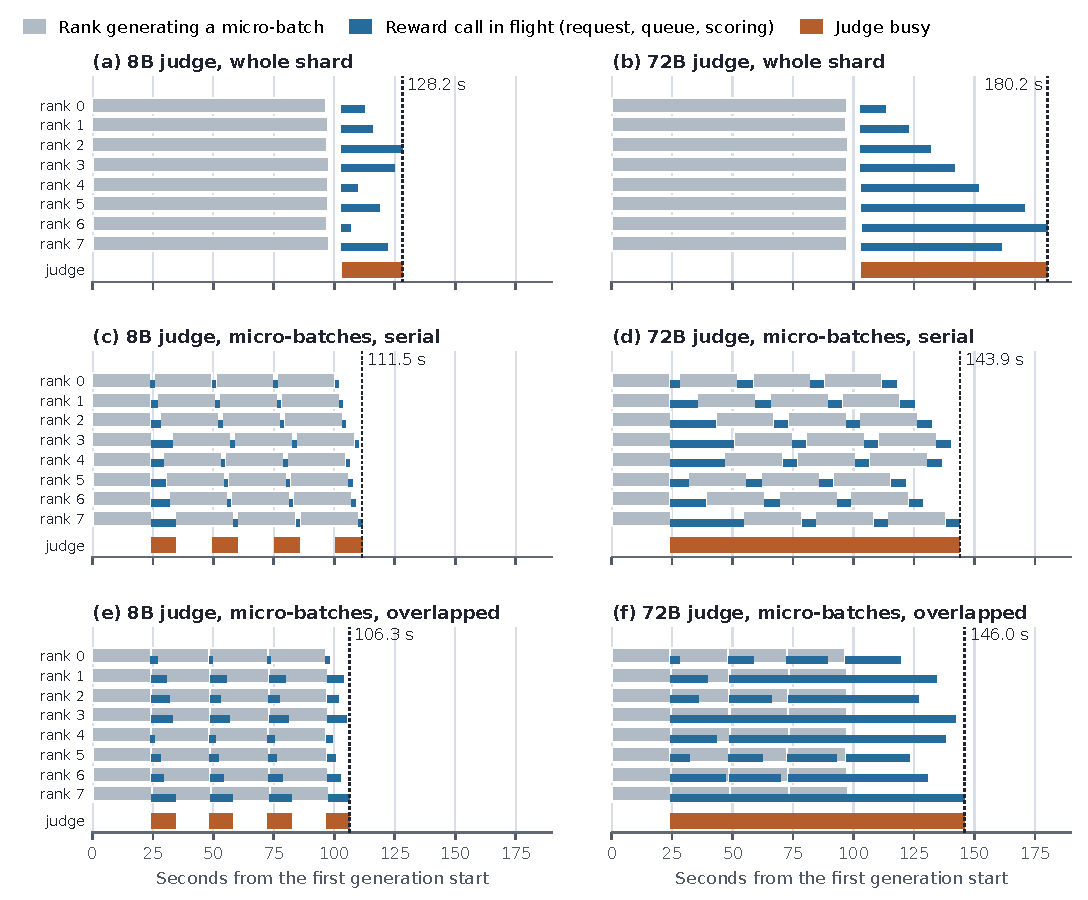
\includegraphics[width=\textwidth]{artifacts/reported_results/2026-09-30-reward-service/figures/overlap_timeline.pdf}
\caption{Recorded rollouts under the three schedules, for the 8B judge (left) and the 72B judge (right). Each panel is the second rollout of one traced run; its rows are the eight ranks of the training node and the judge. Grey is the generation of a micro-batch (of the whole shard in the top row), blue a reward call between request and response, orange the judge at work; the dashed line marks the last score. Times count from the first generation start of that rollout, so they differ slightly from the pooled phase-timer means of Table~\ref{tab:reward-overlap}.}
\label{fig:reward-timeline}
\end{figure}

\begin{table}[H]
\caption{Generation plus reward wall-clock per rollout under three schedules: mean and range over steady-state rollouts. Editing rows use BAGEL with a remote EditScore judge; the last block is BAGEL text-to-image with an in-process PickScore. Overlapped rows pool the merged implementation, which queues every score, with an earlier prototype that kept at most one score in flight; the bundle reports them separately.}
\label{tab:reward-overlap}
\centering
\small
% Generated by artifacts/reported_results/2026-09-30-reward-service/generate.py; do not edit.
\begin{tabularx}{\textwidth}{@{}Xrrrr@{}}
\toprule
Schedule & Rollouts & Generate + reward (s) & Range (s) & vs.\ whole shard \\
\midrule
\multicolumn{5}{@{}l}{EditScore 8B, remote node} \\
Whole shard, driver-dispatched reward & 4 & 126.8 & 125.9--127.8 & -- \\
Micro-batches, serial & 5 & 111.5 & 110.9--111.9 & $-$12.1\% \\
Micro-batches, overlapped & 7 & 106.9 & 106.6--107.3 & $-$15.7\% \\
\midrule
\multicolumn{5}{@{}l}{EditScore 72B, remote node} \\
Whole shard, driver-dispatched reward & 2 & 179.7 & 179.2--180.1 & -- \\
Micro-batches, serial & 4 & 145.0 & 144.4--146.0 & $-$19.3\% \\
Micro-batches, overlapped & 6 & 146.3 & 144.3--149.1 & $-$18.6\% \\
\midrule
\multicolumn{5}{@{}l}{PickScore, in-process} \\
Whole shard, driver-dispatched reward & 2 & 56.0 & 56.0--56.0 & -- \\
Micro-batches, serial & 2 & 52.4 & 52.4--52.5 & $-$6.3\% \\
Micro-batches, overlapped & 2 & 52.3 & 52.3--52.3 & $-$6.5\% \\
\bottomrule
\end{tabularx}

\end{table}

\paragraph{A judge with headroom.}
With the 8B judge, serial micro-batches reduce generation plus reward from \RSSmallBase{}\,s to \RSSmallSerial{}\,s (\RSSmallSerialSaving{}), and overlapping reduces it to \RSSmallOverlap{}\,s (\RSSmallOverlapSaving{}).
Generation itself takes about 98\,s in every arm (Figure~\ref{fig:reward-overlap}); the schedules differ in where the reward time falls (Figure~\ref{fig:reward-timeline}, left).
After a whole shard, the eight requests arrive together and the server scores them one at a time, \RSSmallWholeService{}\,s each, so the last rank waits \RSSmallWholeWaitMax{}\,s for a score that took the judge three.
With serial micro-batches the ranks collide only once, on their first micro-batch, where the longest wait is \RSSmallSerialFirstWaitMax{}\,s.
The unequal waits leave the ranks staggered, and each later request finds the judge free and returns in about \RSSmallSerialLaterWait{}\,s.
With overlap, generation never waits, so the ranks stay in step and collide on every micro-batch; those waits now run beside the next micro-batch's generation, and only the last one remains after generation ends.
The judge is idle for about \RSSmallOverlapIdle{}\,s between its first and its last request, and that headroom is what overlap uses.

\paragraph{A saturated judge.}
With the 72B judge, serial micro-batches reduce generation plus reward from \RSLargeBase{}\,s to \RSLargeSerial{}\,s (\RSLargeSerialSaving{}), and the overlapped schedule is indistinguishable from the serial one: \RSLargeOverlap{}\,s, with a range of \RSLargeOverlapMin{}--\RSLargeOverlapMax{}\,s against \RSLargeSerialMin{}--\RSLargeSerialMax{}\,s.
In both, the judge works without a gap from the arrival of the first micro-batch, \RSLargeFirstArrival{}\,s into the rollout, until its last request (Figure~\ref{fig:reward-timeline}, right).
The rollout therefore ends at that arrival plus the judge's total work, whatever order the requests come in.
That work was \RSLargeSerialWorkMin{}--\RSLargeSerialWorkMax{}\,s per traced rollout under the serial schedule and \RSLargeOverlapWorkMin{}--\RSLargeOverlapWorkMax{}\,s under the overlapped one, and it drifts by two to three seconds between consecutive rollouts of one arm, so the few seconds between the two rows of Table~\ref{tab:reward-overlap} are not an effect of the schedule.
Once the judge is busy for the whole rollout, adding judge capacity or making its requests cheaper is the remaining lever.

\begin{figure}[H]
\centering
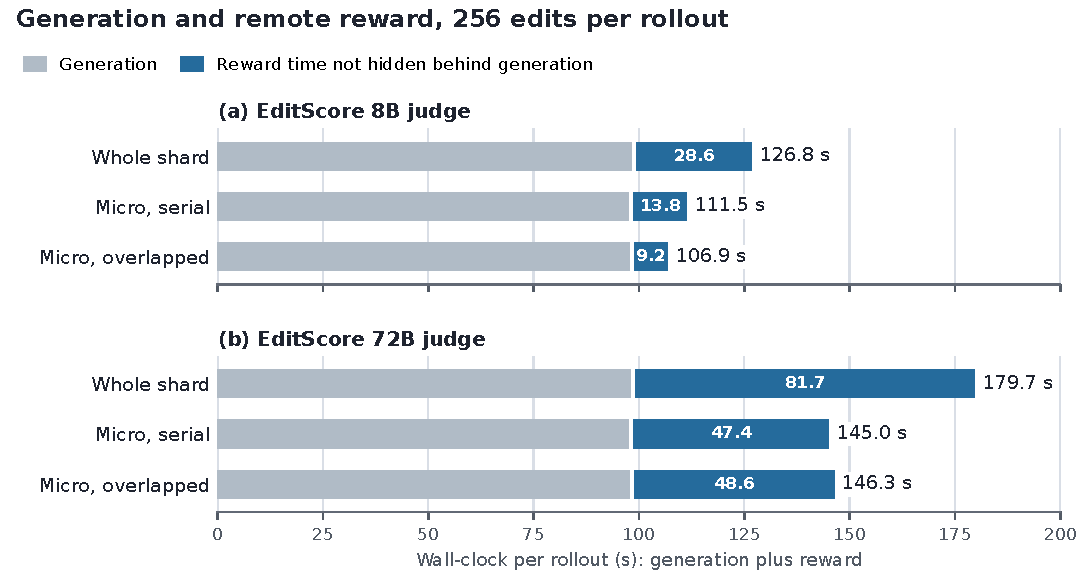
\includegraphics[width=0.85\textwidth]{artifacts/reported_results/2026-09-30-reward-service/figures/overlap_wallclock.pdf}
\caption{Where the rollout's wall-clock goes for the two remote judges of Table~\ref{tab:reward-overlap}. Generation is unchanged by the schedule; the schedules differ in how much reward time remains outside it.}
\label{fig:reward-overlap}
\end{figure}

\paragraph{The price of small requests.}
Micro-batching increases the judge's work.
An eight-pair request costs the 72B judge \RSLargeSerialService{}\,s and a 32-pair request \RSLargeWholeService{}\,s, so a rollout scored in micro-batches needs \RSLargeSerialWork{}\,s of judge time against \RSLargeWholeWork{}\,s for whole shards; for the 8B judge the figures are \RSSmallMicroWork{}\,s and \RSSmallWholeWork{}\,s.
The schedule wins because that work starts a quarter of the way into generation instead of after it, not because there is less of it.
Smaller requests without the stack only pay the price: in a shallower shape with 16 rows per rank, splitting the whole-shard request into eight-row requests was slower than the baseline on both judges (\RSSmallShallowBase{}\,s to \RSSmallShallowSplit{}\,s and \RSLargeShallowBase{}\,s to \RSLargeShallowSplit{}\,s), whereas two micro-batches per rank were faster (\RSSmallShallowSerial{}\,s and \RSLargeShallowSerial{}\,s).
The single-scorer server scores one request at a time; a judge that batched across concurrent requests would recover this cost.

\paragraph{An in-process scorer.}
With PickScore in the policy's workers, reward is a small part of the rollout, and the stack reduces generation plus reward from \RSLocalBase{}\,s to \RSLocalSerial{}\,s.
Scoring inside the worker took about one second in these runs; the rest of the baseline's reward phase is the driver-dispatched call.
Overlap has nothing left to hide here.

\paragraph{A side effect on training.}
The micro-batch loop leaves garbage in the worker's Python heap.
When the following train phase started without a collection pass, it took \RSTrainRemoteNoCollect{}\,s in the 8B-judge runs and \RSTrainLocalNoCollect{}\,s in the PickScore runs; with a pass at the rollout boundary it took \RSTrainRemoteCollect{}\,s and \RSTrainLocalCollect{}\,s.
The merged role therefore collects once the shard has left the worker.
The cost of a rollout schedule has to be read off the whole step, not the rollout phase alone.

\subsection{Sharing one GPU among small scorers}
\label{sec:reward-mps}

The standalone service gives every scorer actor whole devices.
That is simple and isolates faults, but a panel of small preference models leaves most of a large accelerator idle.
Ray can place several actors on one device through fractional resources; the fraction is scheduling bookkeeping, and the separate CUDA processes it co-locates are time-sliced.
NVIDIA's Multi-Process Service (MPS) lets kernels from different processes run concurrently~\citep{nvidiamps}, which keeps one process, and one dependency set, per scorer while using the idle capacity between their kernels.

The open pull request adds this as an opt-in runtime.
The service either owns the MPS daemon of its node, starting it before any actor creates a CUDA context and stopping it after the last one has exited, or attaches to a daemon owned by the platform.
Each reward may set an active-thread percentage and a device-memory allocation cap, which are exported to its actor before its first CUDA call.
The configuration is rejected when it combines sharing with tensor-parallel scorers, with scorers that have not been qualified, or with half-precision weights below a full active-thread share.
Shutdown stops admission, waits for submitted GPU work, and only then terminates actors and the daemon.
The cap limits what a client may allocate; it is not memory isolation, and all clients of one device share a fault domain, which the health endpoint reports.

\begin{table}[H]
\caption{Throughput gain (\%) of MPS over fractional sharing without MPS for two or three copies of one scorer on a single H20, as reported in pull request \#492; $b$ is the model batch. Dashes mark batch sizes at which the scorer does not run one batched forward of that size.}
\label{tab:reward-mps}
\centering
\small
% Generated by artifacts/reported_results/2026-09-30-reward-service/generate.py; do not edit.
\begin{tabular}{@{}lrrrrrr@{}}
\toprule
 & \multicolumn{3}{c}{Two copies} & \multicolumn{3}{c}{Three copies} \\
\cmidrule(lr){2-4}\cmidrule(l){5-7}
Scorer & $b{=}1$ & $b{=}4$ & $b{=}8$ & $b{=}1$ & $b{=}4$ & $b{=}8$ \\
\midrule
CLIP & $+$11.2 & $+$20.0 & $+$14.8 & $+$16.5 & $+$24.4 & $+$19.2 \\
HPSv2 & $+$17.4 & -- & -- & $+$48.4 & -- & -- \\
ImageReward & $+$24.0 & -- & -- & $+$40.8 & -- & -- \\
HPSv3 & $+$20.6 & $+$11.2 & -- & $+$22.6 & $+$12.8 & -- \\
GOT-OCR & $-$2.8 & -- & -- & $-$3.2 & -- & -- \\
\bottomrule
\end{tabular}

\end{table}

\paragraph{Reported results.}
Table~\ref{tab:reward-mps} transcribes the author's qualification on H20 GPUs; we did not repeat it.
For panels of different scorers on one device, the pull request reports a median gain of \RSMpsThreeLight{} for three light scorers and \RSMpsTwoLight{} for two, smaller gains when a heavier vision--language scorer bounds the panel, and none for an autoregressive OCR scorer.
Scores were identical with and without MPS on its deterministic fixture.
The gain comes from filling idle device time between the kernels of different processes; the pull request's profiles put a single CLIP process at about half of the device's time at batch one.
It is a utilization result for small models and does not add capacity once one scorer saturates the device.

\paragraph{A correctness boundary.}
The same qualification found that an active-thread percentage below 100 produced wrong half-precision matrix products on the tested H20 driver stack: non-finite CLIP scores, and finite but incorrect PickScore values.
The runtime therefore refuses half-precision scorers below a full share.
A reviewer did not reproduce the failure on a different accelerator and driver, where the same panel was bound by CPU and HTTP work and co-location cost almost nothing even without MPS.
The benefit and the hazard both depend on the device and driver, and a throughput figure from one stack should not be carried to another.
Only CLIP and PickScore at a full share are qualified in the pull request; vision--language judges, longer soak runs, and sharing a device between reward and the policy's own roles are outside its scope.
